\begin{flushright}
    \textit{Лекция 14 (от 20.10)}
\end{flushright}
\section{$\S 18.$ Вычисление интегралов от регулярных ветвей.}
\Example
Вычислить при помощи теории вычетов интеграл
\begin{align*}
  & I = \int_0^2 \frac{\sqrt[4]{x^3(2-x)}}{(1+x)^2} dx
\end{align*}
\nonum
$g(z) = \sqrt[4]{z^3(2-z)}$ дает многозначную функцию. Отыщем регулярные ветви;
рассмотрим область, где ветви существуют. Функция $f(z) = z^3(2-z)$ должна быть
в области регулярной и не равной нулю.
\\
Рассмотрим $\CC \setminus [0;2]$. В такой области этот корень имеет регулярную
ветвь.
\\
Отыщем ветвь, что нам нужна. Построим ее так, чтобы $g(1+i0) = 1$; тогда
$\forall x \in [0;2] \ g(x+i0) = \sqrt[4]{x^3(2-x)}$. В этом случае
\begin{align*}
  & g(x-i0) = g(1+i0)\exp\left( \frac{i}{4}\left( 3\Delta_{\gamma_{1+i0,x}}\argt z + \Delta_{\gamma_{1+i0,x}}\argt (2-z) \right) \right) = \exp\left( \frac{-i\pi}{2}\right)
\end{align*}
\begin{figure}[h!]
		\centering
		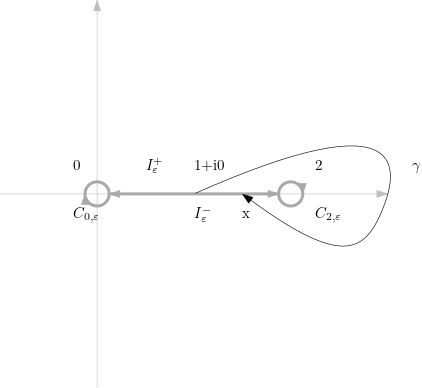
\includegraphics[scale=0.5]{Par18.png}
		\label{fig:18.1}
\end{figure}
Рассмотрим
\begin{align*}
  & \gamma_\varepsilon = I_\varepsilon^+\cup C_{2, \varepsilon} \cup I_\varepsilon^-\cup C_{0, \varepsilon}
\end{align*}
и
\begin{align*}
  & F(z) = \frac{\sqrt[4]{z^3(2-z)}}{(1+z)^2} = \frac{g(z)}{(1+z)^2}
\end{align*}
и вычислим
\begin{align*}
  & I_\varepsilon = \int_{\gamma_\varepsilon}F(z) dz = 2 i \pi \left( \us{-1}{\res} F(z) + \us{\infty}{\res} F(z) \right)
\end{align*}
Видим, что $-1$~--- полюс $2$ порядка, а $\infty$~--- УОТ.
\begin{align*}
  & \us{-1}{\res} F(z) = \lim_{z \to -1}((z+1)^2F(z))' = \lim_{z \to -1}g'(z) = g'(-1) = \frac{f'(z)}{4g^3(z)}\mid_{z = -1} = \frac{-4(-1)^3+6(-1)^2}{4\left( \sqrt[4]{3}\exp\left( \frac{3i\pi}{4} \right)\right)^3} = \\
  & = \frac{5}{2\sqrt[4]{27}}\exp\left( \frac{-i\pi}{4} \right)
\end{align*}
Рассмотрим $x \in (2; \infty)$; тогда
\begin{align*}
  & g(x) = \sqrt[4]{x^3(2-x)}\exp\left( \frac{-i\pi}{4} \right) = x\sqrt[4]{1-\frac{2}{x}}\exp \left( \frac{-i\pi}{4} \right) = x\exp\left( \frac{-i\pi}{4} \right)\sum_{n=0}^\infty C_{\frac{1}{4}}^n\left( -\frac{2}{x} \right)^n
\end{align*}
Две регулярные функции ($g(x)$ и сумма) совпадают на $(2; \infty)$, а значит, по
теореме единственности
\begin{align*}
  & g(z) = z\exp\left( \frac{-i\pi}{4} \right)\sum_{n=0}^\infty C_{\frac{1}{4}}^n\left( -\frac{2}{z} \right)^n, \ \left| z \right|> 2
\end{align*}
\begin{align*}
  & F(z) = \frac{z}{(z+1)^2}h(z), \ h(z) = \exp\left( \frac{-i\pi}{4} \right)\sum_{n=0}^\infty C_{\frac{1}{4}}^n\left( -\frac{2}{z} \right)^n
\end{align*}
Заметим, что
\begin{align*}
  & \frac{z}{(1+z)^2} = \frac{1}{z(1+\frac{1}{z})^2} = \frac{1}{z} \left( 1-\frac{2}{z} +\frac{3}{z^2} + \dots \right)
\end{align*}
При перемножении двух рядов получим
\begin{align*}
  & \us{\infty}{\res}F(z) = -\exp\left( \frac{-i\pi}{4} \right)
\end{align*}
и интеграл
\begin{align*}
  & I_\varepsilon = 2 i \pi \left( \frac{5}{2\sqrt[4]{27}} - 1 \right)\exp\left( \frac{-i\pi}{4} \right)
\end{align*}
не зависит от $\varepsilon$. Заметим, что
\begin{align*}
  & I_\varepsilon = \int_{I_\varepsilon^+}F(z) + \int_{C_{2, \varepsilon}}F(z) + \int_{I_\varepsilon^-}F(z) + \int_{C_{0, \varepsilon}}F(z)
\end{align*}
Причем
\begin{align*}
  & \int_{I_\varepsilon^+}F(z) = \int_{\varepsilon}^{2-\varepsilon}\frac{\sqrt[4]{x^3(2-x)}}{(x+1)^2}dx
\end{align*}
\begin{align*}
  & \int_{I_\varepsilon^-}F(z) = \int_{2-\varepsilon}^{\varepsilon}\frac{g(x-i0)}{(x+1)^2}dx = -\int_{\varepsilon}^{2-\varepsilon}\frac{\sqrt[4]{x^3(2-x)}\exp\left( \frac{3i\pi}{2} \right)}{(x+1)^2}dx = -\exp\left( \frac{3i\pi}{2}\right) \int_{I_\varepsilon^+}F(z)
\end{align*}
Учтя $z = \varepsilon e^{i \varphi}$,
\begin{align*}
  & \left|  \int_{C_{0, \varepsilon}}F(z) \right| \leq \int_{0}^{2 \pi}\frac{\sqrt[4]{\varepsilon^3(2+\varepsilon)}\varepsilon}{(1-\varepsilon)^2}d\varphi \leq A\varepsilon^{\frac{7}{3}} \us{\varepsilon \to 0}{\to} 0
\end{align*}
Учтя $z = 2 + \varepsilon e^{i \varphi}$,
\begin{align*}
  & \left|  \int_{C_{2, \varepsilon}}F(z) \right| \leq \int_{0}^{2 \pi}\frac{\sqrt[4]{(2+\varepsilon)^3\varepsilon}\varepsilon}{(3-\varepsilon)^2}d\varphi \leq B\varepsilon^{\frac{4}{3}} \us{\varepsilon \to 0}{\to} 0
\end{align*}
Значит,
\begin{align*}
  & 2 i \pi \left( \frac{5}{2\sqrt[4]{27}} - 1 \right)\exp\left( \frac{-i\pi}{4} \right) = I_\varepsilon \us{\varepsilon \to 0}{\to} \int_{I_\varepsilon^+}F(z) + \int_{I_\varepsilon^-}F(z) = \left( 1 -\exp\left( \frac{3i\pi}{2}\right) \right) \int_{I_\varepsilon^+}F(z) \us{\varepsilon \to 0}{\to} \\
  & \us{\varepsilon \to 0}{\to} \left( 1 -\exp\left( \frac{3i\pi}{2}\right) \right) I
\end{align*}
Значит,
\begin{align*}
  & I = \frac{2 i \pi \left( \dst \frac{5}{2\sqrt[4]{27}} - 1 \right)\exp\left( \dst\frac{-i\pi}{4} \right)}{\left( 1 -\exp\left( \dst \frac{3i\pi}{2}\right) \right)}= \pi \sqrt{2}\left( \dst \frac{5}{2\sqrt[4]{27}} - 1 \right)
\end{align*}
\section{$\S 19.$ Целые и мероморфные функции.}
